\documentclass[12pt]{article}
\usepackage{geometry}                % See geometry.pdf to learn the layout options. There are lots.
\geometry{letterpaper}                   % ... or a4paper or a5paper or ... 
\usepackage{graphicx}
\usepackage{amssymb}
\usepackage{amsthm}
\usepackage{epstopdf}
\usepackage[utf8]{inputenc}
\usepackage[usenames,dvipsnames]{color}
\usepackage[table]{xcolor}
\usepackage{hyperref}
\usepackage{float}
\usepackage[inline]{enumitem}
\hypersetup{
    colorlinks=true,
    linkcolor=blue,
    filecolor=magenta,      
    urlcolor=cyan,
}
\usepackage{parskip}
\DeclareGraphicsRule{.tif}{png}{.png}{`convert #1 `dirname #1`/`basename #1 .tif`.png}

\theoremstyle{definition}
\newtheorem{example}{Example}

\newenvironment{explanation}{%
   \setlength{\parindent}{0pt}
   \itshape
   \color{blue}
}{}

\newcommand{\projectname}{Doctor Robert}
\newcommand{\productname}{Doctor Robert}
\newcommand{\projectleader}{D. Weidinger}
\newcommand{\documentstatus}{In process}
%\newcommand{\documentstatus}{Submitted}
%\newcommand{\documentstatus}{Released}
\newcommand{\version}{V. 1.0}

\begin{document}
\begin{titlepage}
\begin{flushright}
\end{flushright}

\vspace{10em}

\begin{center}
{\Huge System Specifications} \\[3em]
{\LARGE \productname} \\[3em]

\includegraphics[scale=.5]{logo.png}\\
\end{center}

\vspace{10em}

\begin{flushleft}
\begin{tabular}{|l|l|}
\hline
Project Name & \projectname \\ \hline
Project Leader & \projectleader \\ \hline
Document state & \documentstatus \\ \hline
Version & \version \\ \hline
\end{tabular}
\end{flushleft}

\end{titlepage}

\section*{Revisions}
\begin{tabular}{|l|l|l|}
\hline
\cellcolor[gray]{0.5}\textcolor{white}{Date} & \cellcolor[gray]{0.5}\textcolor{white}{Author} & \cellcolor[gray]{0.5}\textcolor{white}{Change} \\ \hline
November 08, 2019& Gruber, Tanzer, Weidinger &Initial Situation \\ \hline
November 15, 2019& Gruber, Tanzer, Weidinger & Use Cases\\ \hline
November 18, 2019& Gruber, Tanzer, Weidinger &Use Cases \\ \hline
November 22, 2019& Gruber, Tanzer, Weidinger &Use Cases, Application Domain \\ \hline
November 29, 2019& Gruber, Tanzer, Weidinger &Use Cases, NFR \\ \hline
November 06, 2019& Gruber, Tanzer, Weidinger &NFR \\ \hline
November 13, 2019& Gruber, Tanzer, Weidinger &Quantity Structure, System Architecture \\ \hline
November 16, 2019& Gruber, Tanzer, Weidinger & Patching  \\ \hline
November 20, 2019& Gruber, Tanzer, Weidinger &Proof Reading\\ \hline
\end{tabular}
\pagebreak

\tableofcontents
\pagebreak

\section{Initial Situation and Goal}

\subsection{Initial Situation}

When people start to show symptoms of a possible sickness or get mildly injured, they often tend to misjudge or downplay the severity of their conditions, to justify not making a doctors appointment, since going to the doctors is a big inconvenience for most people in this day of age. This behaviour often leads those people to seek out to google for a diagnosis.

Googling symptoms can be quite tedious and unnecessarily time-consuming. It involves opening a lot of sites, skimming trough loads of text and most of the time the results are rather inaccurate. 

Although there are already good individual solutions for medical third opinions, there has yet to be a simple unified platform for all individual cases.
{\bf For example} \href{https://www.netdoktor.de/}{Netdoktor}, the market leader for medical articles and questions in German speaking countries, has a program called \href{https://www.netdoktor.de/symptom-checker/}{Symptom-Checker} that tries to simplify the process of searching for medical treatments on their own website by asking the user questions about their gender, age, area of pain, etc. This process also includes redundant questions and limits the user to input only by selection, which makes it hard to accurately describe symptoms. Netdoktor only supports the German language so if a user wants an English diagnosis they have to switch to a different service.

Such services also lack features like scanning skin in order to diagnose skin diseases, so a user has to use, or even download, another application like for example \href{http://www.skinvision.com}{Skin Vision}, which is a program used to recognize skin diseases based on images. This could lead the user to not look up their suspicious looking piece of skin. 

As of now we are not aware of any healthcare assistants or symptom checkers that make use of sophisticated Artificial Intelligence algorithms. Neuronal networks trained on medical data, like BioBert, already exist and outperform established solutions in regards of accuracy and convenience but are not easily accessible for the ordinary consumer.

Additionally, we want to provide medical professionals the opportunity to profit from our platform by placing location based advertisements. Depending on the type of problem or injury, advertisements will be selected to match the needs of the user and refer to the right kind of professional. 

To make advertising more appealing to potential advertisers we want to collect anonymous statistical data. Doctors then can see if placing an advertisement would be beneficial for their business. For example, a chiropractor could promote their ordination in an area with an higher likely hood of back problems.

We also realized how much impact an improvement in the online healthcare consultation actually has. Every second citizen of Austria at least once googled their complains. An estimated amount of 70.000 of google's queries per minute, spread all over the world, are health related.

\pagebreak

\subsubsection{Application Domain}

Our system, in its core, is a healthcare assistant. As a healthcare assistant, your job is to provide information and advice for those who need it. Therefore our system acts in a way that information given by a user is converted to a corresponding answer/advice. 

It is base upon an NLP model (natural language processing model). NLP is a sub field of linguistic and artificial intelligence concerned with the interaction between humans and computers via natural language. This model on its own cannot be used in a practicable way. It has to be wrapped in a shell like, for instance, a mobile application to make it available for commercial use. Applications programs or groups of programs designed for end users with an UI(user interface) for user interaction and UX(user experience) for the usage feeling.

Next to being a health care assistant, the system also includes an advertising portal for medical professionals and pharmaceutical companies. With Medical professionals we mean doctors, chiropractors and other certified personnel allowed to care out medical tasks who want to attract potential customers to their ordinations or rather businesses. Whereas pharmaceutical companies can use the opportunity to advertise their drugs.


\subsubsection{Glossary}

\begin{itemize}
    \item healthcare assistant
    
    Someone or something that provides information or rather assists someone regarding health and healthcare. 
    
    \item healthcare
    
    is the maintenance or improvement of health via the prevention, diagnosis, treatment, recovery, or cure of disease, illness, injury, and other physical and mental impairments in people.
    
    \item NLP
    
    Short for natural language processing which is a sub field of linguistic and artificial intelligence concerned with the interaction between humans and computers via natural language.
    
    \item artificial intelligence
    
    is intelligence demonstrated by machines, in contrast to the natural intelligence displayed by humans.
    
    \item linguistic
    
    is the scientific study of language. It involves analysing language form, language meaning, and language in context.
    
    \item (mobile) application
    
    is a program or group of programs designed for end users. In our case, the application is deployed for mobile devices.
    
    \item UI
    
    Short for User Interface. The UI describes the space of operation between human and computer.
    
    \item UX
    
    Short for User Experience. It is concerned with a person's emotions and attitudes about using a particular product, system or service.
    
    \item advertisement
    
    Advertising is a marketing communication that employs an openly sponsored, non-personal message to promote or sell a product, service or idea.
    
    \item advertising portal
    
    An application to access advertisement functionality. Like booking ads or reviewing statistics regarding placed ads. For instance the number of people you reached or those who already click on the ads.
    
    \item medical professional
    
    Someone who is certified or legally allowed to carry out medical tasks.
    
    \item doctor
    
    A medical professional who has a degree in medicine or a sub field of medicine.
    
    \item pharmaceutical companies
    
    Companies whose main source of income comes from the distribution and creation of drugs.
    
    \item ordination
    
    Synonym to doctor's office or in a broader sense a medical professional's office.
    
\end{itemize}

\subsubsection{Model of the Application Domain}

This section gives an high-level overview of our application domain.

\begin{figure}[H]
    \centering
    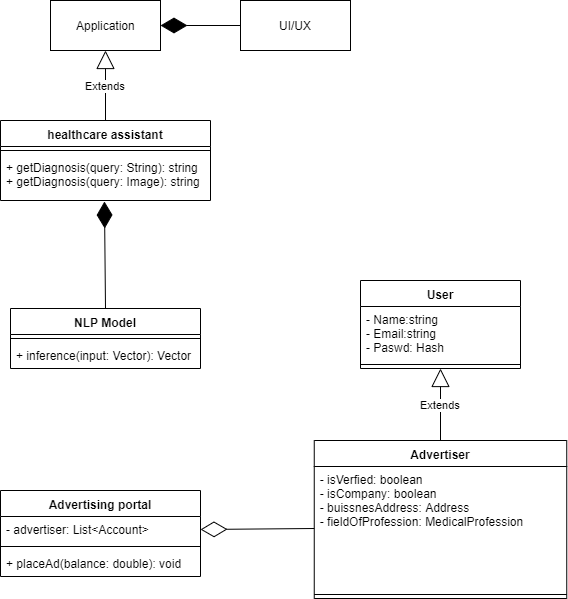
\includegraphics[scale=0.6]{SystemSpec/Usecases/Diagrams/DoctorRobert-ClassDiagram.png}
    \caption{high-level representation of the application domain}
    \label{fig:my_label}
\end{figure}

\pagebreak

\subsection{Goal}

Our main goal is to provide medical advice, such as a specific diagnosis to a certain illness or a suggestion to see a professional. By using an outstandingly trained neural-network we can supply thoroughly in-depth and yet simple answers to what the user has to know about his current state. If the diagnosis shows indication of skin irritations, it automatically suggests a skin scan for a higher quality analysis. In case the response is a tiny bit too complex, redirects for further explanations and links to qualified websites are provided.
Additionally, we allocate marketing space for medical professionals like doctors or even accomplished medical companies by placing advertisements of the respected advertiser. The advertisements are placed based on raised statistics of our given diagnoses, consisting of certain keywords, how often and where they are used, giving advertisers the chance to target the right area of possible customers and maximise their profit.

\pagebreak

\section{Functional Requirements}

\subsection{Overview}

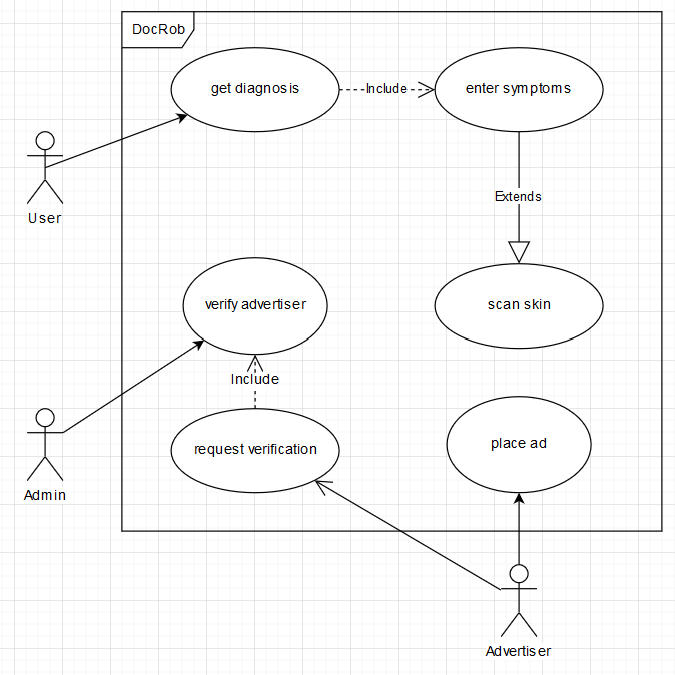
\includegraphics[scale=1.69420]{SystemSpec/Usecases/Diagrams/UseCaseDiagram.png}\\

\begin{enumerate*}
    \item Get Diagnosis,
    \item Enter Symptoms,
    \item Scan Skin,
    \item Place ad,
    \item Request verification
    \item Verify advertiser
\end{enumerate*}

\subsection{UI Overview}

\begin{minipage}{0.4\textwidth}
\begin{figure}[H]
\centering
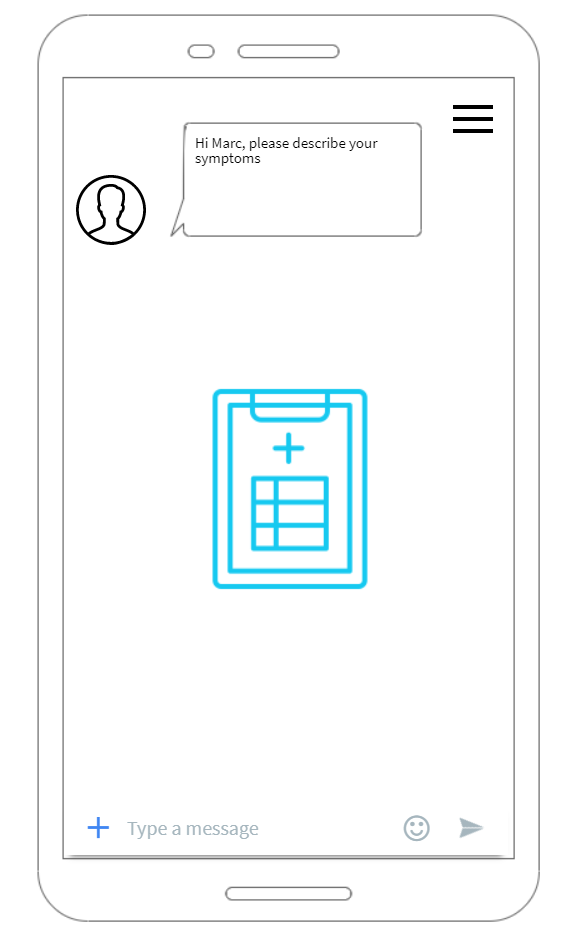
\includegraphics[scale=.8]{SystemSpec/Usecases/Mocks/MockOverview.PNG}\\
\caption{\label{fig:blue_rectangle} main page}
\end{figure}
\end{minipage} \hfill
\begin{minipage}{0.6\textwidth}

The user enters his ailments into the app. Using words or whole sentences to describe the current unwell-feeling. Since the predication will be more accurate if more keywords are read, a more precise description of the
illness is better than just words. Even though words alone are sufficient.

The output informs the user about possible symptoms causing the ill-being and/or about feasible solution and if desired further elaboration on certain results.

The user then can decide how to act from that point. Depending on the outcome he can leave it be, do further research through provided links or arrange a doctors appointment.

\end{minipage}

\pagebreak

\subsection{Use Case 1: Enter symptoms}
\subsubsection{General Description}

\begin{tabular}{|p{.2\linewidth}|p{.65\linewidth}|}
\hline 
ID: & EnterSymptoms \\ \hline
Goal: & The user enters a description/keywords of their complaints for further analyzing. \\ \hline
Precondition: & - \\ \hline
Postcondition: & Get Diagnosis is executed. \\ \hline
Involved Users: &User: Someone who uses our system. \\ \hline
\end{tabular}

\subsubsection{UI to call the use case}
\begin{minipage}{0.4\textwidth}
\begin{figure}[H]
\centering
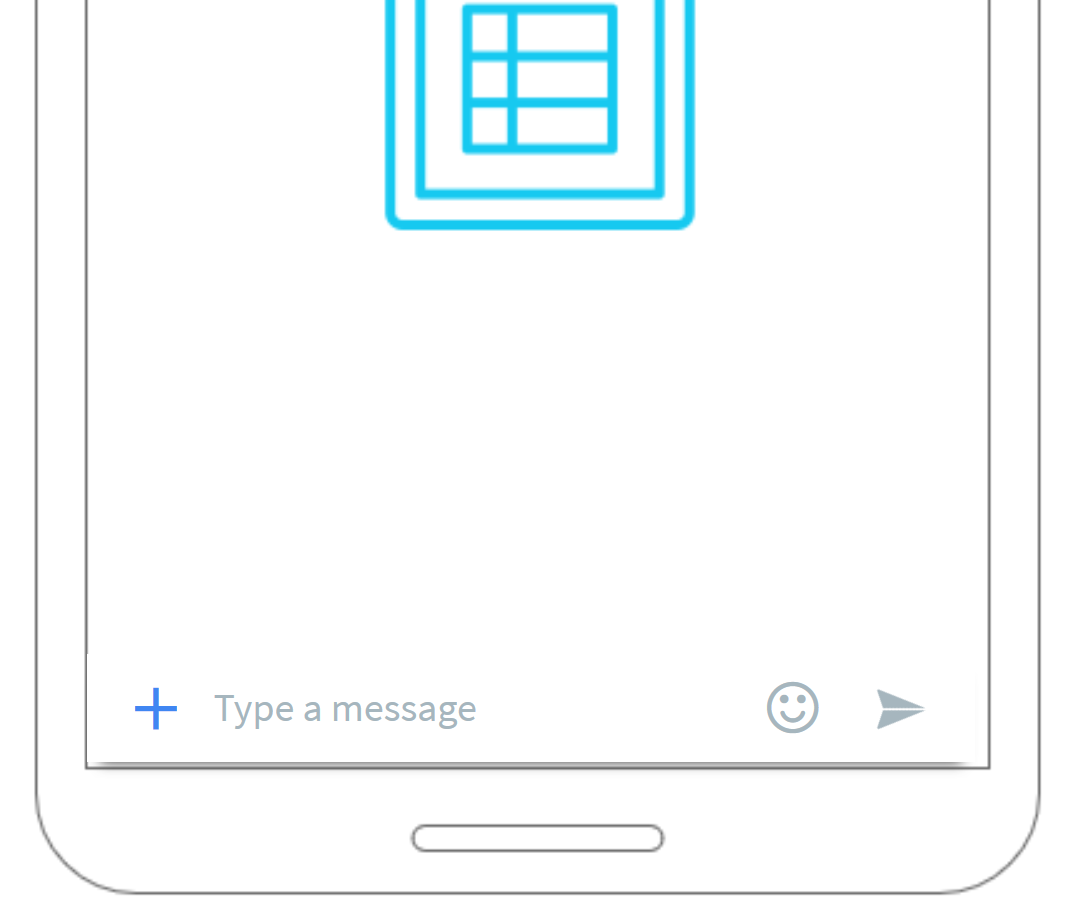
\includegraphics[scale=.4]{SystemSpec/Usecases/Mocks/entersym01.png}\\
\caption{\label{fig:blue_rectangle}enter symptoms}
\end{figure}
\end{minipage} \hfill
\begin{minipage}{0.6\textwidth}
The Dialog-Bar is used to describe your complaints and confirm said message.
\end{minipage}


\subsubsection{The Standard Use}
\begin{minipage}{0.4\textwidth}
\begin{figure}[H]
\centering
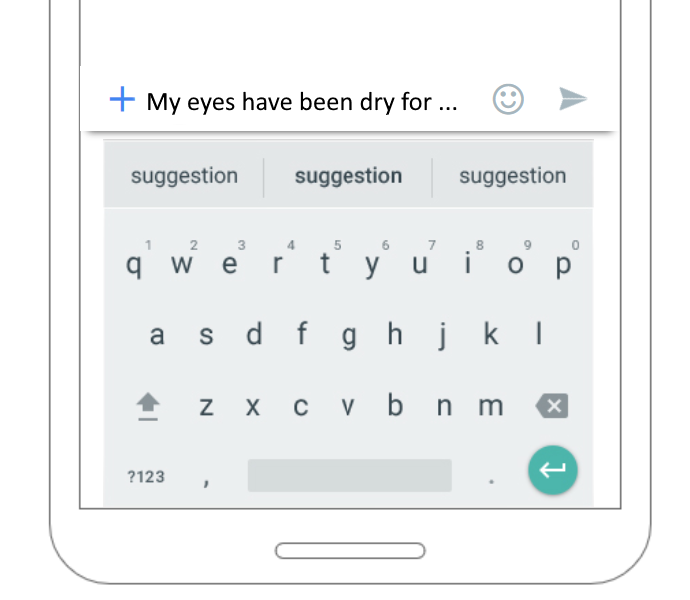
\includegraphics[scale=.27]{SystemSpec/Usecases/Mocks/entersym02Normal.png}\\
\caption{\label{fig:blue_rectangle}enter symptoms}
\end{figure}
\end{minipage} \hfill
\begin{minipage}{0.6\textwidth}
The user opens app, selects the Dialog-Bar enters his ailments into the app. Using words or whole sentences to describe the current malady.
\end{minipage}

\begin{figure}[H]
\begin{center}
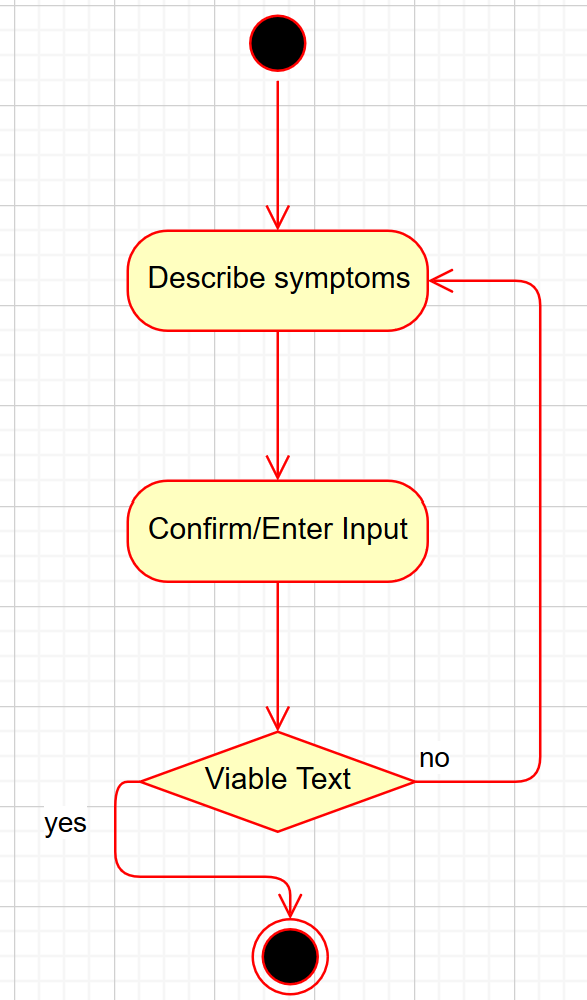
\includegraphics[scale=1]{SystemSpec/Usecases/Diagrams/entersymActivity.png}\\
\caption{\label{fig:blue_rectangle}enter symptoms}
\end{center}
\end{figure}

\subsubsection{The Non-Standard Use}
\begin{minipage}{0.4\textwidth}
\begin{figure}[H]
\centering
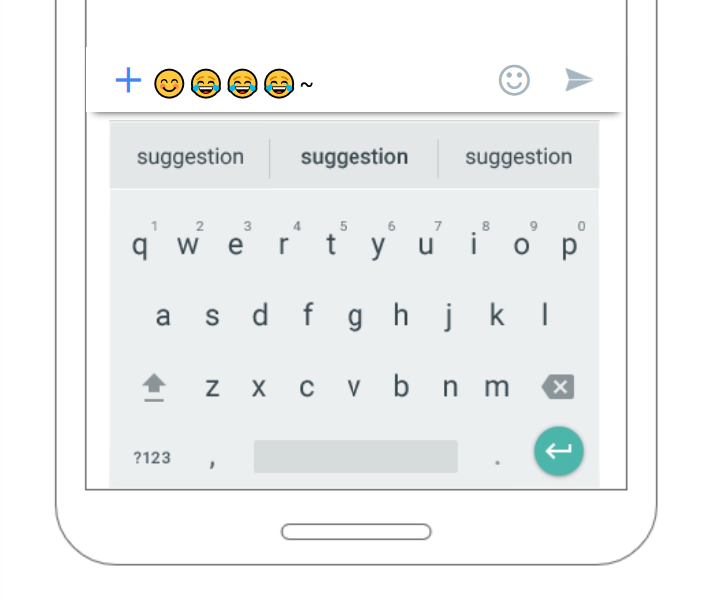
\includegraphics[scale=.7]{SystemSpec/Usecases/Mocks/entersym02Non.png}\\
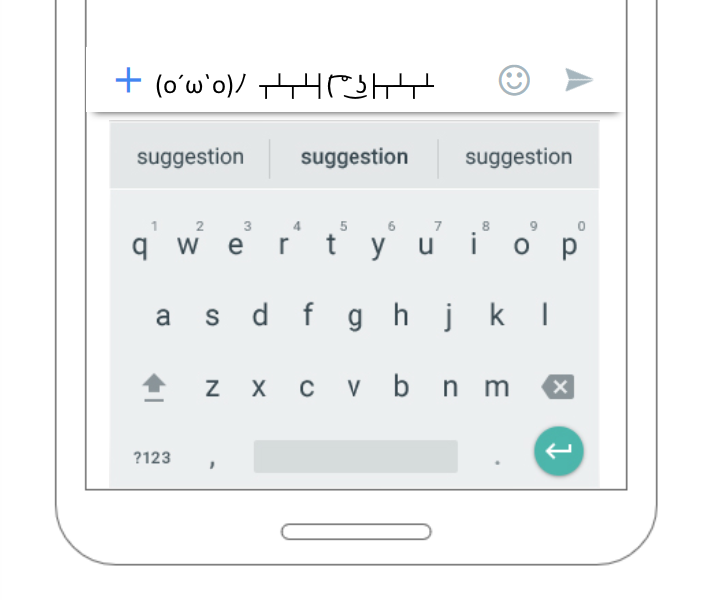
\includegraphics[scale=.7]{SystemSpec/Usecases/Mocks/entersym02NonAscii.png}\\
\caption{\label{fig:blue_rectangle}enter symptoms}
\end{figure}
\end{minipage} \hfill
\begin{minipage}{0.6\textwidth}
The user's input is not applicable. Before the input is transmitted to our back-end it will be checked for, for instance, senseless text like emojis or UNI-Code characters that are not used in languages. The input will be ignored and not further processed and the user will receive an error message.
\end{minipage}

\pagebreak


\subsection{Use Case 3: Scan Skin}

    \subsubsection{General Description}
    
        \begin{tabular}{|p{.2\linewidth}|p{.65\linewidth}|}
        \hline 
        ID: & Scan Skin \\ \hline
        Goal: & To let the user submit a picture so an diagnosis can be made \\ \hline
        Precondition: & The user selected the Scan Skin feature from the burger menu or it got recommend in the chat based on an previous diagnosis  \\ \hline
        Postcondition: & The user can now get an diagnosis based on their picture \\ \hline
        Involved Users: & User:  Someone who uses our app \\ \hline
        \end{tabular}
    
    \subsubsection{UI to call the use case}
        
        There are two ways a user can open our skin scan feature:
        
        \begin{enumerate}
        \item The user opens our app with the intent to check their skin and starts the process of getting a diagnosis by clicking on the menu icon and selecting the camera icon to start taking a picture and submitting it.
            
            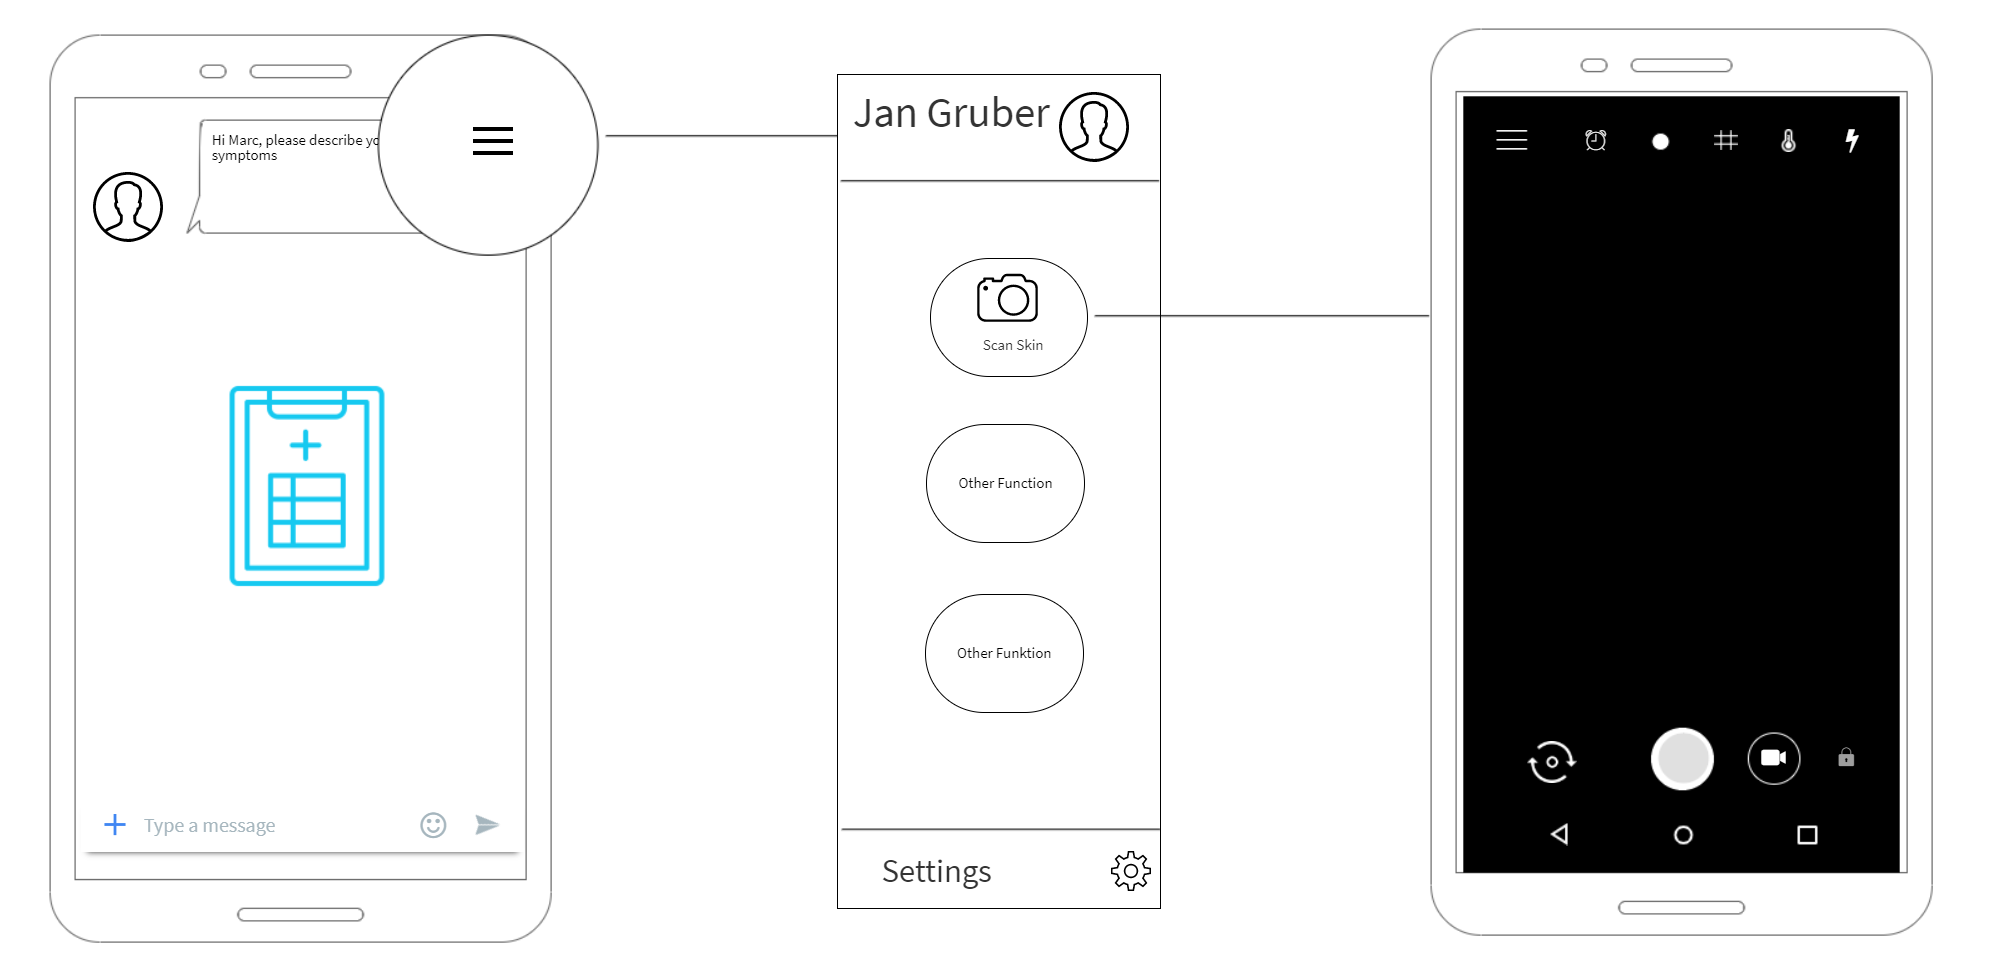
\includegraphics[scale=0.7]{SystemSpec/Usecases/Mocks/scanskin01.png}\\
        
        \item The user has already entered their somewhat skin related symptoms, so to make the diagnosis more accurate Doctor Robert suggests to try our skin scan feature and provides an option to open it right from the dialog.
        
            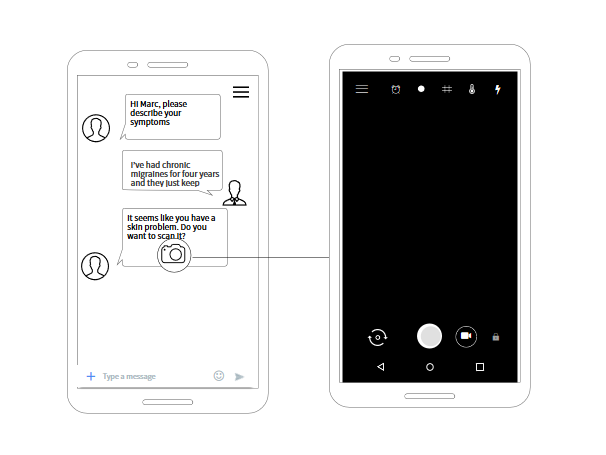
\includegraphics[scale=0.7]{SystemSpec/Usecases/Mocks/scanskin02.png}\\
            
        \end{enumerate}
    
    \subsubsection{The Standard Use}
        
        Depending on how the use case was called the happy path differs a bit, but is essentially the same:
        
       \begin{center}
            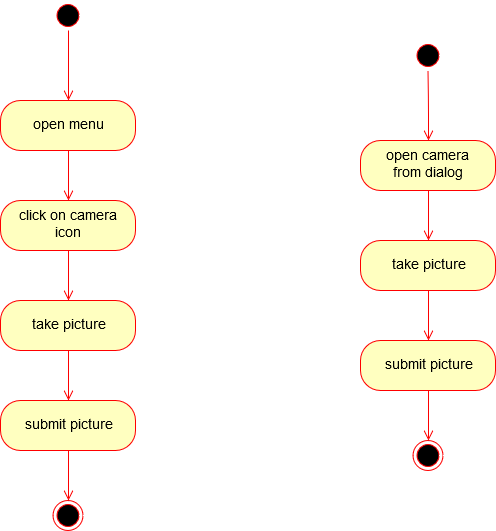
\includegraphics[scale=0.49]{SystemSpec/Usecases/Diagrams/ScanSkinActivity1.png}\\
       \end{center}{}
        
        \paragraph{open menu}
        The user clicks on the menu button and the burger menu opens.
        
        \paragraph{click on camera icon}
        The user clicks on the camera icon to open the camera.
        
        \paragraph{open camera from dialog}
        The user clicks on a button provided in the dialog from Doctor Robert, to open the camera.
        
        \paragraph{take picture}
        The user takes a picture.
        
        \paragraph{submit picture}
        The user submits the picture he took by pressing a button.
    
    \subsubsection{The Non-Standard Use}
        
        \begin{itemize}
            \item The user submits a picture of something other than skin.
            
                This is specified in \hyperlink{ScanSkinNonStandard}{GetDiagnosis}
        \end{itemize}{}
        
\pagebreak


\subsection{Use Case 2: Get Diagnosis}

 \subsubsection{General Description}
\begin{tabular}{|p{.2\linewidth}|p{.65\linewidth}|}
\hline 
ID: & Get Diagnosis \\ \hline
Goal: & The user gets the diagnosis for their individual complains \\ \hline
Precondition: &  The user entered their symptoms via text or scanned their skin via our skin scanning feature\\ \hline
Postcondition: & The user gets their diagnosis \\ \hline
Involved Users: & User: Someone who uses our app \\ \hline
\end{tabular}

\subsubsection{UI}

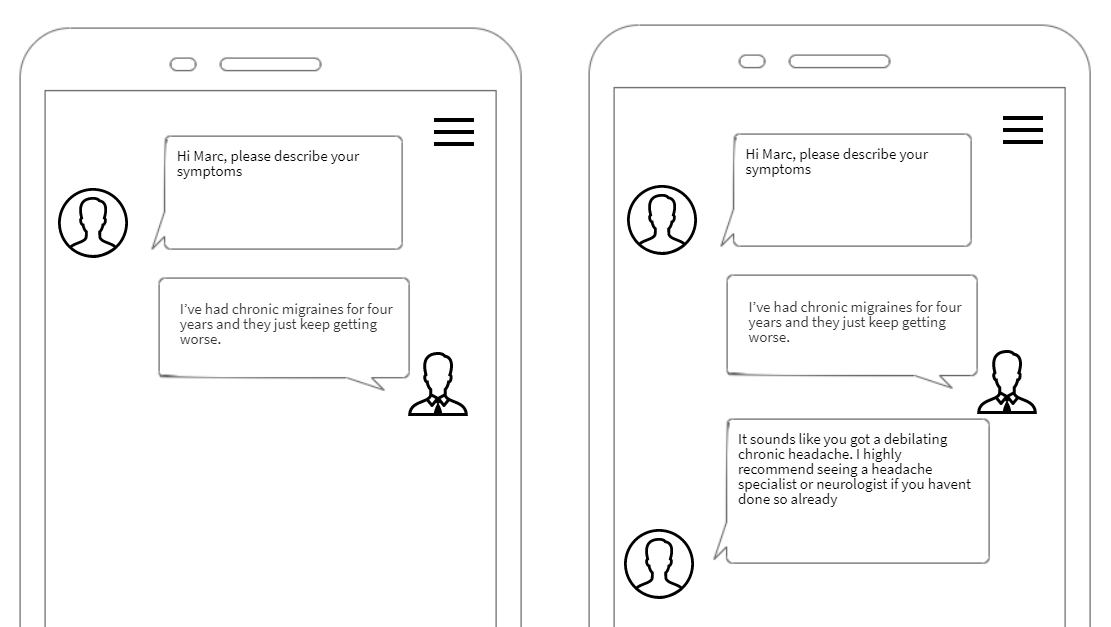
\includegraphics[scale=1.2]{SystemSpec/Usecases/Mocks/getdiagnosis01.PNG}\\
The user receives their diagnosis in form of an chat message from DoctorRobert after they entered their symptoms. If the answer contains any complicated medical terms, DoctorRobert will simplify it and provide further reading material regarding the complicated terms.

\subsubsection{The Standard Use}
\begin{figure}[H]
\centering
    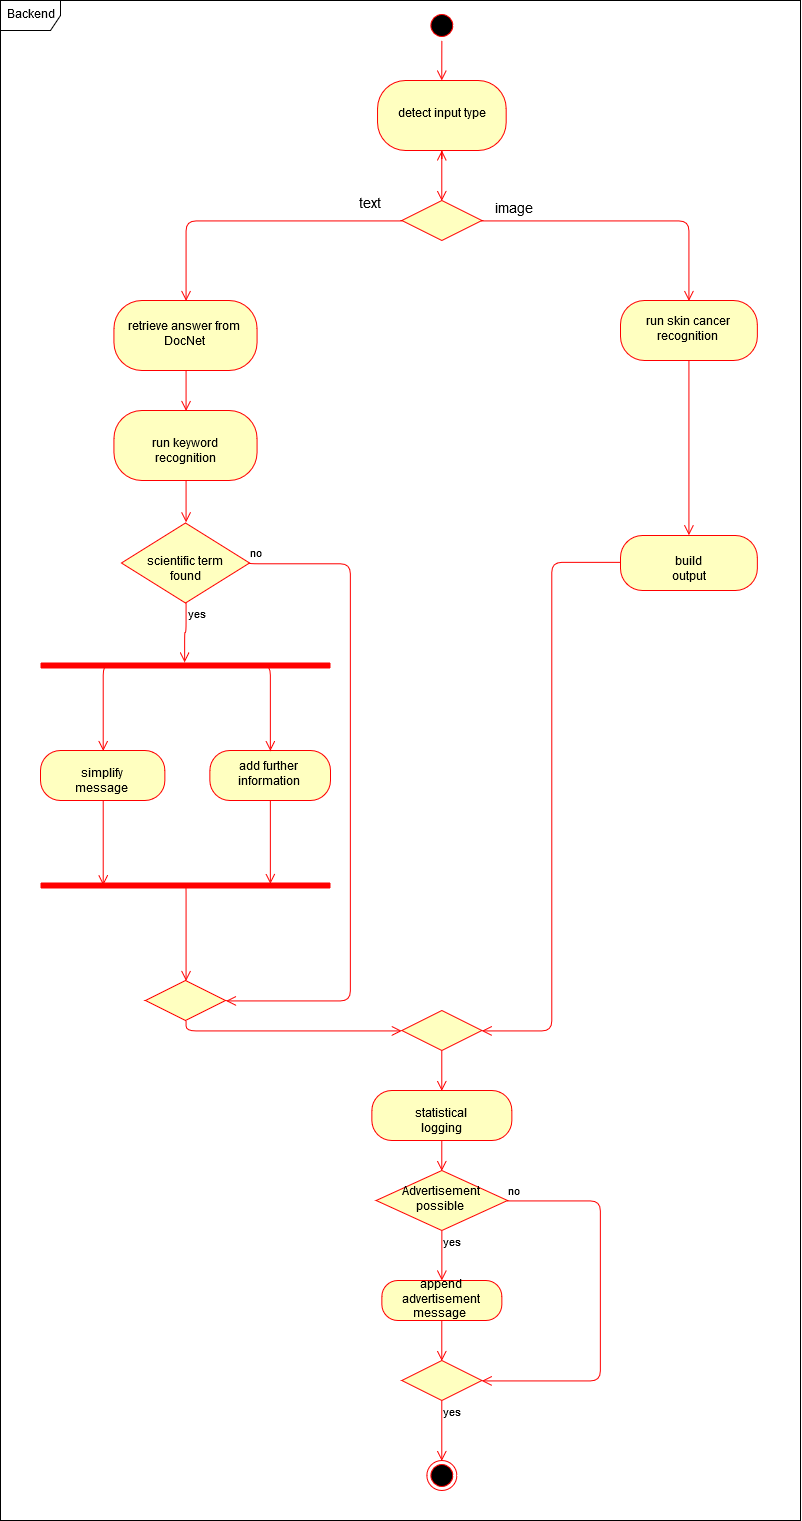
\includegraphics[scale=0.32]{SystemSpec/Usecases/Diagrams/GetDiagnosisActivity.png}
\caption{\label{fig:blue_rectangle}get diagnosis activity}
\end{figure}

\paragraph{detect input type}
Our back-end will determine whether the input is entered in the form of a text or as a picture.

\paragraph{retrieve answer from DocNet}
The input will run trough our AI algorithm and an response will be generated.

\paragraph{run keyword recognition}
The generated response from activity "retrieve answer from DocNet" will be checked for certain keywords.

\paragraph{scientific term found}
If the keyword recognition finds terms which are too scientific or hard to understand, the two use cases "simplify message" and "add further information" will be triggered. 

\paragraph{simplify message}
Based on the keyword recognition an algorithm tries to simplify and make the final response more readable.

\paragraph{add further information}
Based on the keyword recognition certain keywords will receive explanations so a user can understand them. This will be realised by hyperlinking further reading material to the word.

\paragraph{run skin cancer recognition}
If the input is a picture it will run through our computer vision AI. The AI will determine a percentage of how confident it is that the user has skin cancer. This result will be used to create an diagnosis message in "build output".

\paragraph{build output}

A answer will be assembled based on the output of the previous activity.

\paragraph{anonymous logging of data for our advertisement feature}
Before the back-end will send and terminate the message to provide anonymity. We will include relevant data from the answer to the users question in our statistics. This process will only capture data that can not be pin pointed to a specific user. The statistics are used for consumer analysis and marketing purposes.

\paragraph{append advertisement message}

If the final answer to the query(image or text) contains any keywords that match the description of an paying advertiser, an corresponding ad will be shown. \hypertarget{AdIllustration}{An illustration is shown below.}
\begin{center}
    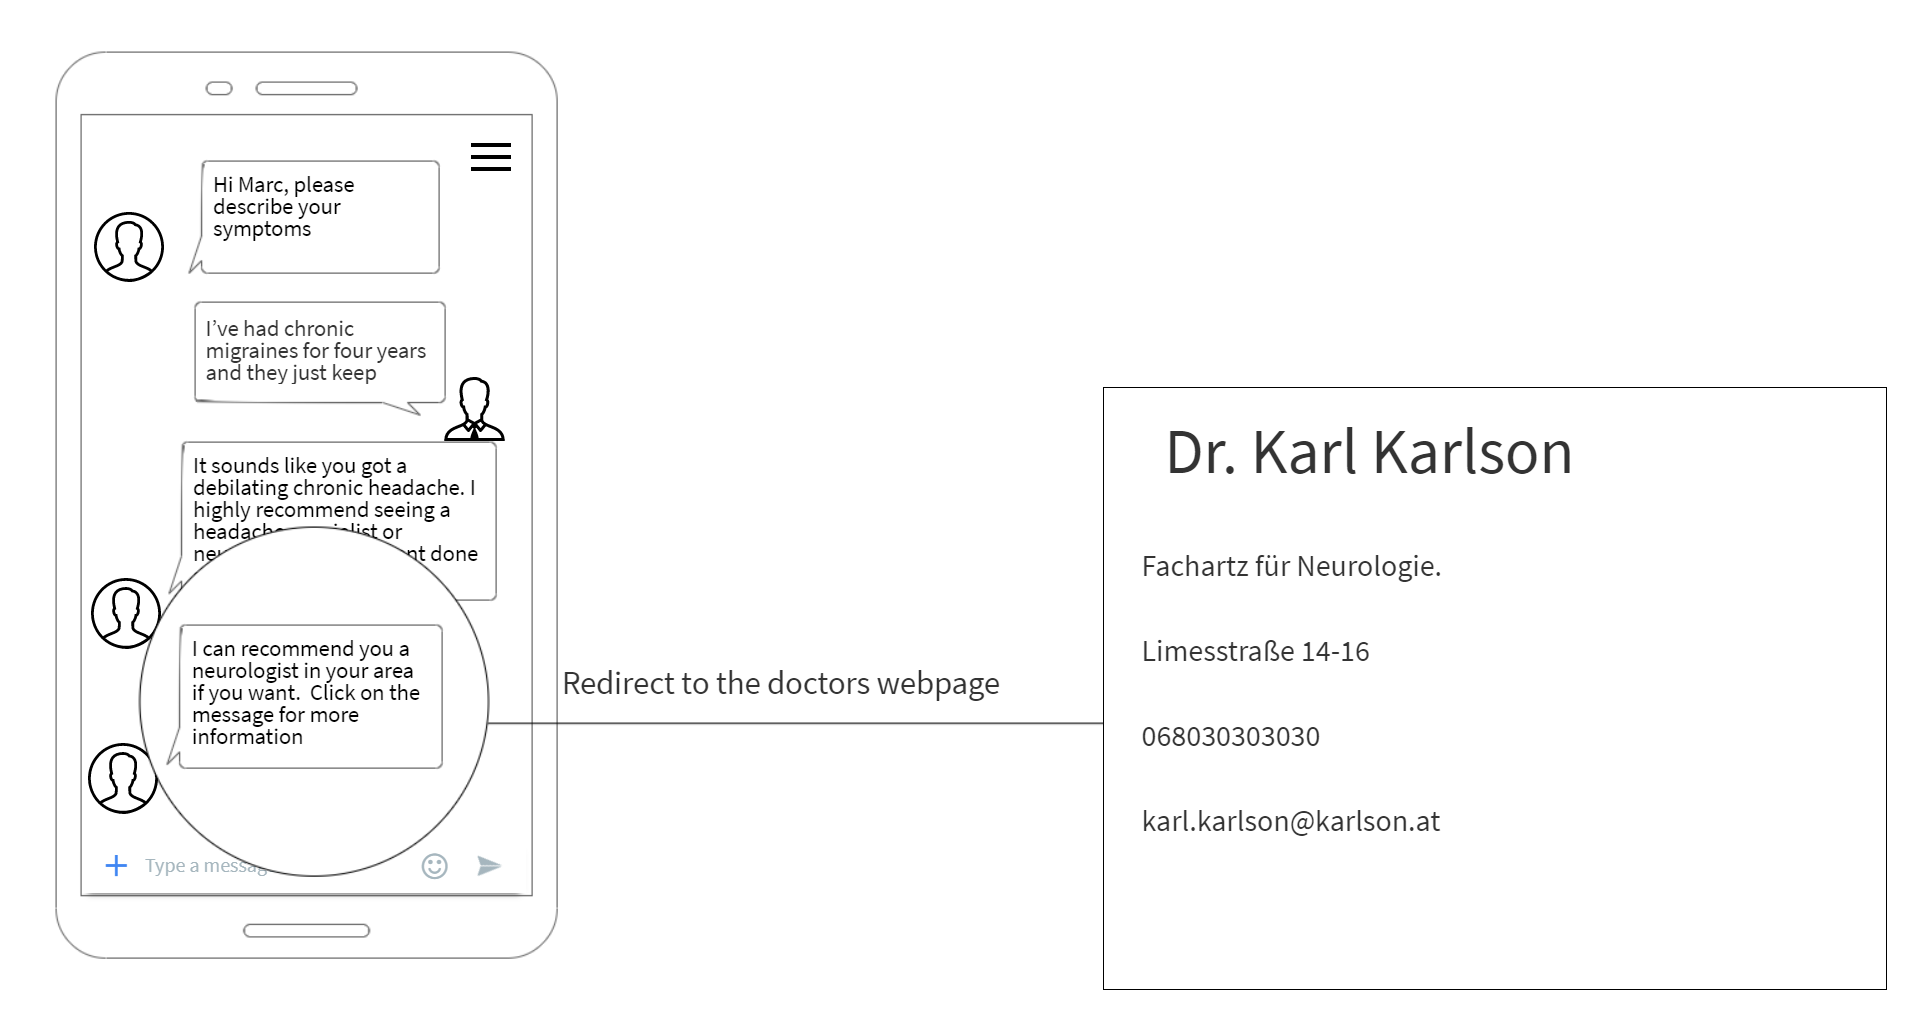
\includegraphics[scale=0.8]{SystemSpec/Usecases/Mocks/advertismentMock.PNG}
\end{center}

\subsubsection{The Non-Standard Use}

\begin{itemize}
    \item User enters something that doesn't make sense
    
    If a user enters nonsensical symptoms or no real  symptoms at all our system will not be able to recognize the fault therefor the input will be treated as normal and the user will receive an equally rubbish answer as their input. 
    
    \item \hypertarget{ScanSkinNonStandard}{The user submits a picture of something other than skin.}
        
        \begin{center}
            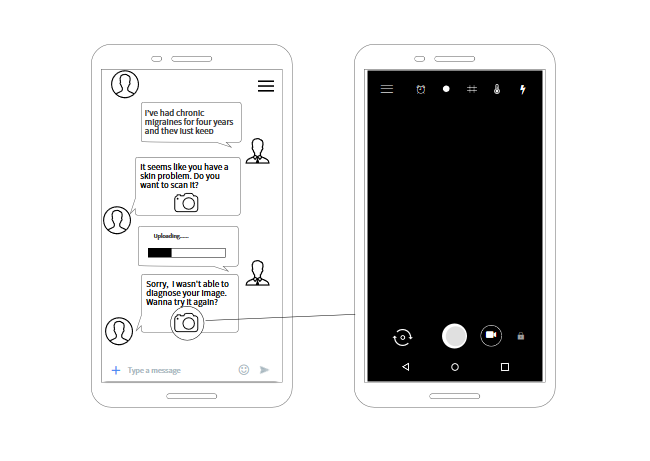
\includegraphics[scale=.7]{SystemSpec/Usecases/Mocks/getdiagnosis02.png}\\
        \end{center}{}
    
        If the percentage of confidence in the diagnosis of our scanning algorithm is too low, like for example when a user submits a faulty image, the user will be asked to take another picture instead of getting an diagnosis like shown above.
    
    \item AI misprediction

    Sometimes the AI is not able to interpret the given query the right way. Unfortunately, we are not able to detect extreme mispredictions yet. In order to avoid the users distrust, measure to clarify this imperfection have to be set. For instance, showing the user a reminder about mentioned imperfections at the start of the application. 

\end{itemize}

\pagebreak


\subsection{Use Case 5: Request Verification}

\subsubsection{General Description}
\begin{tabular}{|p{.2\linewidth}|p{.65\linewidth}|}
\hline 
ID: & Request Verification \\ \hline
Goal: & Get a verified account. \\ \hline
Precondition: & The user must be logged in with an advertiser account.  \\ \hline
Postcondition: & The advertiser can now be approved. \\ \hline
Involved Users: & Advertiser: Portrays doctors, medical companies and so forth, who use the system to place advertisements. \\ \hline
\end{tabular}

\subsubsection{UI to call the use case}
\begin{minipage}{1\textwidth}
\begin{figure}[H]
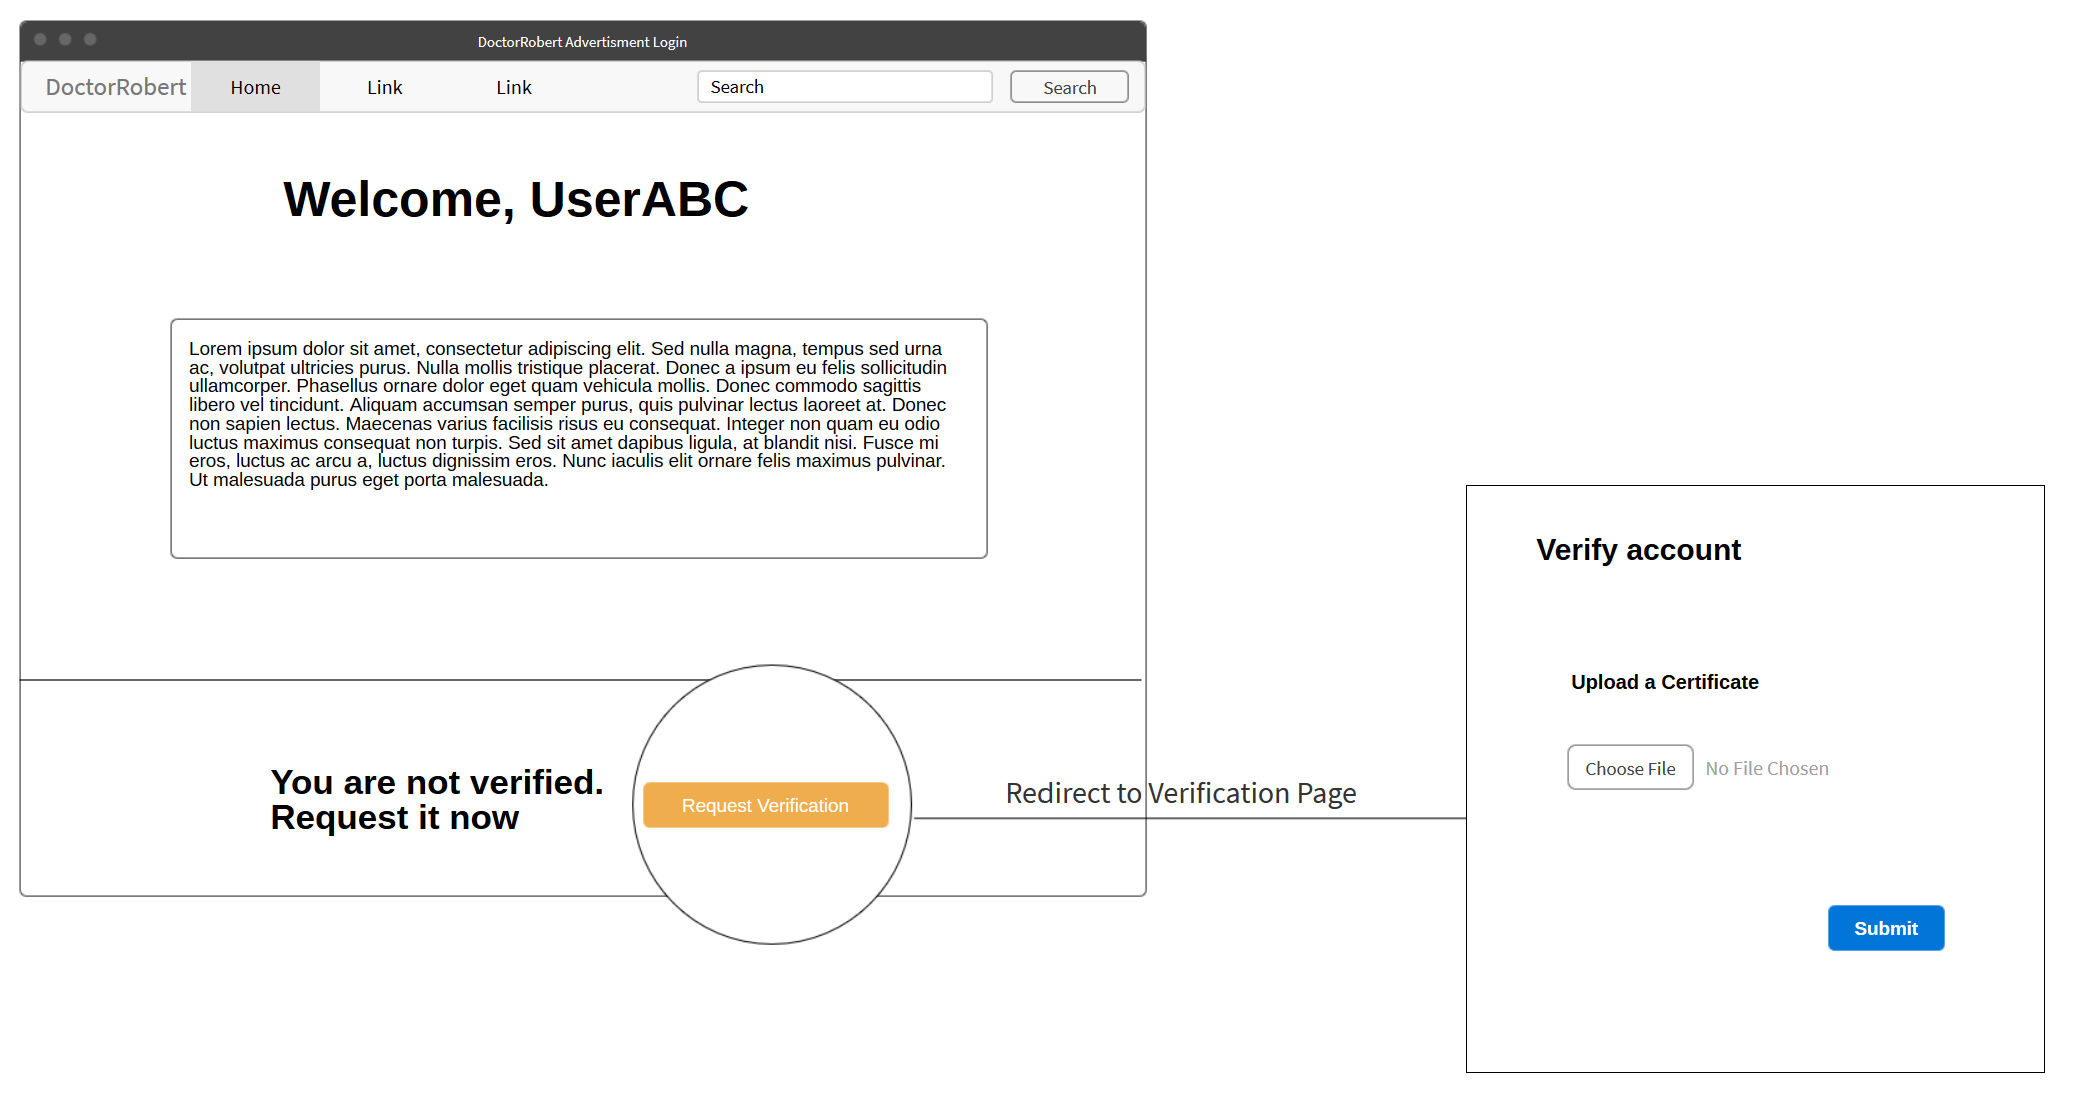
\includegraphics[scale=.65]{SystemSpec/Usecases/Mocks/reqVeri01.png}\\
\caption{\label{fig:blue_rectangle}Request Verification UI}
\end{figure}
\end{minipage} \hfill
\begin{minipage}{1\textwidth}
The advertisement portal will only be available as web application since there is no need for an ordinary customer to access it via the mobile app.
The main screen of an advertiser account gives the option to request verification for this advertiser, by pressing the responsible button, if not already verified. After pressing the "Request Verification"-Button the advertiser has to select two files, one containing some sort of certificate and the second an possible way of identification. For instance a personalized picture containing the contenders face an ID and a handwritten message with a randomly generated message on it.
In the end the files will be sent to us for verification.
\end{minipage}

\subsubsection{The Standard Use}

\begin{minipage}{0.5\textwidth}
\begin{figure}[H]
\centering
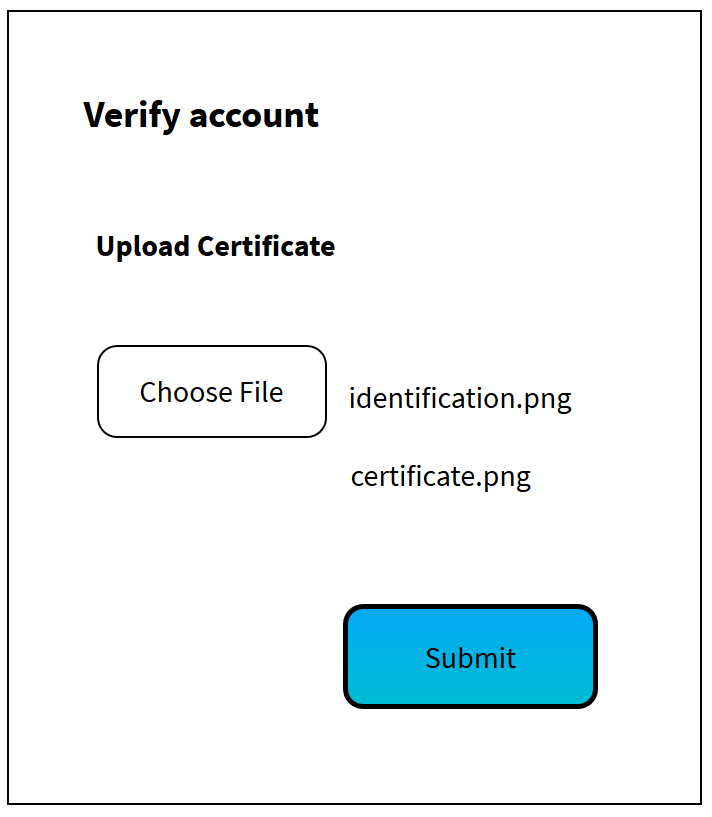
\includegraphics[scale=.8]{SystemSpec/Usecases/Mocks/reqVerNormal.png}\\
\caption{\label{fig:blue_rectangle}Standard Use}
\end{figure}
\end{minipage} \hfill
\begin{minipage}{0.5\textwidth}
The advertiser chooses to upload .png-Files containing a certificate and identification, then submits these for verification.
\end{minipage}

\begin{center}
\begin{figure}[H]
\centering
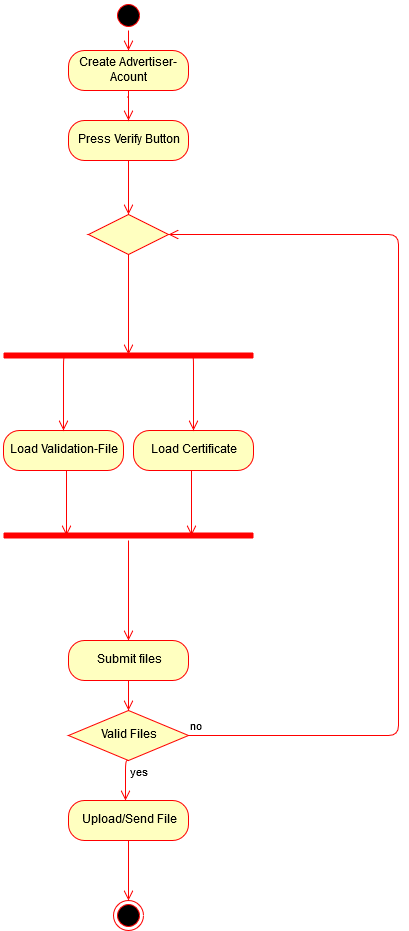
\includegraphics[scale=0.5]{SystemSpec/Usecases/Diagrams/RequestVerificationActivity.png}
\caption{\label{fig:blue_rectangle}Request Verification Activity}
\end{figure}
\end{center}

\subsubsection{The Non-Standard Use}

\begin{minipage}{0.5\textwidth}
\begin{figure}[H]
\centering
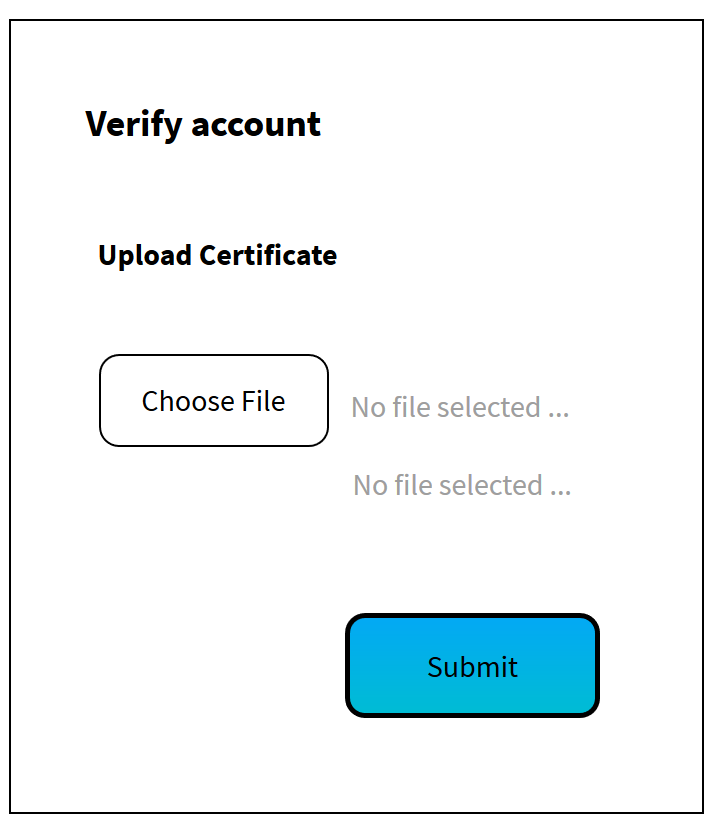
\includegraphics[scale=.6]{SystemSpec/Usecases/Mocks/reqVerNon02.png}\\
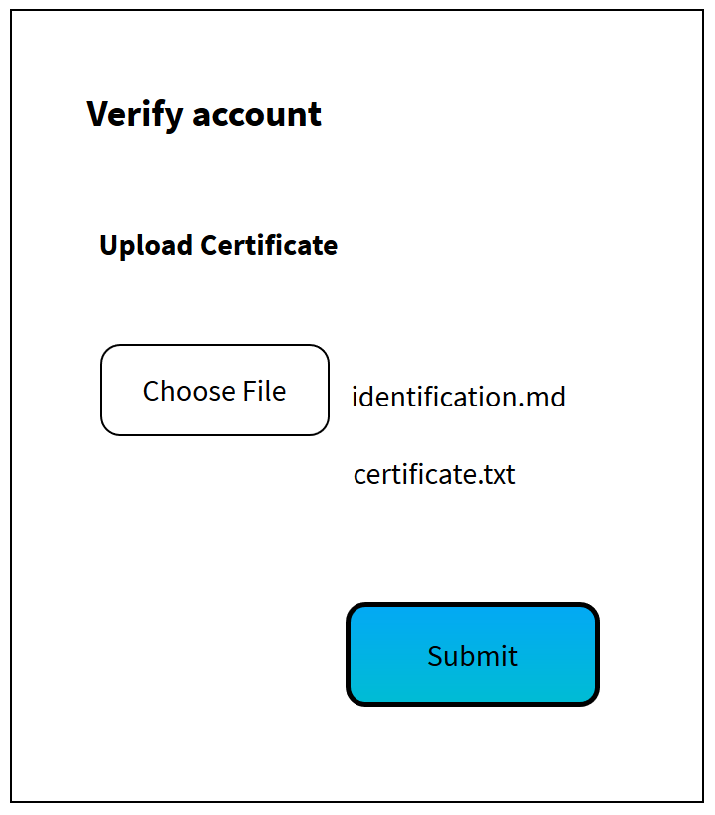
\includegraphics[scale=.6]{SystemSpec/Usecases/Mocks/reqVerNon01.png}\\
\caption{\label{fig:blue_rectangle}Non-Standard Uses}
\end{figure}
\end{minipage} \hfill
\begin{minipage}{0.5\textwidth}
The types of the uploaded files are either of a wrong format, blank empty Files or the advertiser did not select files at all. 
\end{minipage}

\pagebreak


\subsection{Use Case 6: Verify Advertiser}

\subsubsection{General Description}
\begin{tabular}{|p{.2\linewidth}|p{.65\linewidth}|}
\hline 
ID: & Verify Advertiser \\ \hline
Goal: & To process a verification request. \\ \hline
Precondition: & A verification request must have been made.  \\ \hline
Postcondition: & The request either gets accepted and an advertiser account is granted or it gets denied and a rejection message will be sent \\ \hline
Involved Users: & Admin: Somebody who is authorized to verify requests \\ \hline
\end{tabular}

\subsubsection{UI}

After a possible advertiser has made an verification request on our website, the actual authorization process happens personally outside our system and the interaction with the possible advertiser will be handled via email to enable personal message exchange. So this Use Case has no User Interface.

\subsubsection{The Standard Use}

After we receive an verification request, an admin has to personally review the sent certificates and authorization files to either accept the request and grant the advertiser a verified status or deny it and send an rejection message with reasoning on why it will not be accepted.

\subsubsection{The Non-Standard Use}

\begin{itemize}
    \item The request is not serious
    
    If an request is obviously not made with serious intent, it will be ignored and deleted. 
    
    \item We cannot confirm the authenticity of the pictures
    
    If the send verification picture are, for example, low resolution and blurry and are therefor not readable, the admin has to sent an response that urges the possible advertiser to redo the request verification process.
    
\end{itemize}

\pagebreak


\subsection{Use Case 4: Place Ad}

\subsubsection{General Description}

\begin{tabular}{|p{.2\linewidth}|p{.65\linewidth}|}
\hline 
ID: & place ad \\ \hline
Goal: & To enable the promotion of an medical professional, consequently making revenue \\ \hline
Precondition: & A verified advertiser payed for an ad placement \\ \hline
Postcondition: & Advertisements are shown to the user as long as the advertiser pays for it. \\ \hline
Involved Users: & Advertiser: Someone who is verified and has the means to advertise \\ \hline
\end{tabular}

\subsubsection{UI to call the use case}

\begin{center}
\begin{figure}[H]
\centering
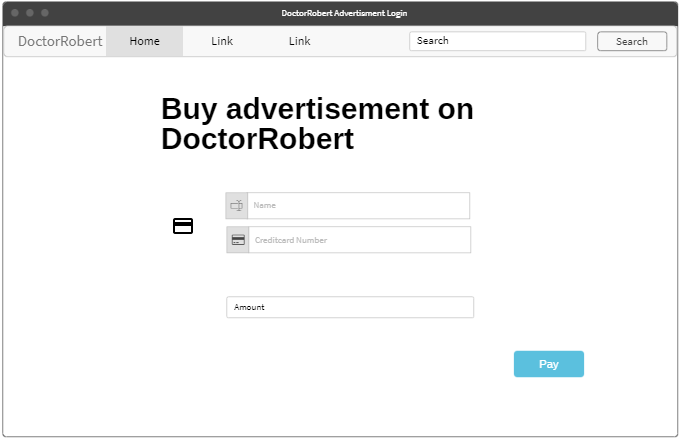
\includegraphics[scale=0.8]{SystemSpec/Usecases/Mocks/placead01.PNG}
\caption{\label{fig:blue_rectangle}Place Ad}
\end{figure}
\end{center}

The advertiser can choose between multiple payment methods. The payment itself will be outsourced to Stripe and PayPal.

\subsubsection{The Standard Use}

If a user is an verified advertiser, he will have the option place advertisements in our app via our website. To place ads the advertiser has to pay us. The amount paid will determine how frequent and how often the ads will be shown. Similar to Google's advertisement model an advertiser pays for one ad and for every time the ad is shown we will charge a small fee and after the whole amount is used the ad will no longer be shown on our app. An appropriate message to inform the advertiser will be sent. One can find an corresponding illustration in the subsection \hyperlink{AdIllustration}{2.4 Use Case 2: Get Diagnosis}



\subsubsection{The Non-Standard Use}

\begin{itemize}
    \item The payment doesn't go through
    
    If the payment doesn't go through, because for example they entered wrong payment information or a trying to scam us, we simply will not show the ad and send the advertiser a rejection message.
    
\end{itemize}

\pagebreak


\section{Non-Functional Requirements}

\subsection{NFR 1: Medical Related Data}
\begin{tabular}{|p{.2\linewidth}|p{.65\linewidth}|}
\hline 
ID: & NFR01 \\ \hline
Name: & Medical Related Data \\ \hline
Type	: & SEC \\ \hline
Description: &  Information regarding the health or general condition of a user must not be saved and secure from third parties.\\ \hline
\end{tabular}

\subsection{NFR 2: AI Ethic}
\begin{tabular}{|p{.2\linewidth}|p{.65\linewidth}|}
\hline 
ID: & NFR02 \\ \hline
Name: & AI Ethic \\ \hline
Type	: & LEGAL \\ \hline
Description: & As for now, experts are not sure about the legal situation of Artificial Intelligence giving medical advice to humans. Therefore, to be on the safe side, we will clearly communicate the user that the solutions the system provides are not in any way a substitute or replacement for a doctor's opinion. \\ \hline
\end{tabular}

\subsection{NFR 3: Clearly laid out answers}
\begin{tabular}{|p{.2\linewidth}|p{.65\linewidth}|}
\hline 
ID: & NFR03 \\ \hline
Name: & Clearly laid out answers \\ \hline
Type	: & USE \\ \hline
Description: & To make sure the diagnoses and responses made by Doctor Robert are neatly laid out, to ensure a good UX, we at most give two responses and automatically clear the chat history when the app closes. \\ \hline
\end{tabular}

\subsection{NFR 4: Reliability}
\begin{tabular}{|p{.2\linewidth}|p{.65\linewidth}|}
\hline 
ID: & NFR03 \\ \hline
Name: & Reliability \\ \hline
Type	: & USE \\ \hline
Description: &  Our diagnoses' and predictions' failure rate has to be lower than 0.05\%.  \\ \hline
\end{tabular}

\subsection{NFR 5: Convenience}
\begin{tabular}{|p{.2\linewidth}|p{.65\linewidth}|}
\hline 
ID: & NFR03 \\ \hline
Name: & Convenience \\ \hline
Type	: & USE \\ \hline
Description: & The whole process of typing in the complaints and getting the diagnosis has to be done in less steps than just googling.  \\ \hline
\end{tabular}

\subsection{NFR 6: Prompt answers}
\begin{tabular}{|p{.2\linewidth}|p{.65\linewidth}|}
\hline 
ID: & NFR03 \\ \hline
Name: & Prompt answers \\ \hline
Type	: & EFFIC \\ \hline
Description: & The response time shall be within 500 ms.  \\ \hline
\end{tabular}

\pagebreak

\section{Quantity Structure}

For the collection of our data we will use firebase, google's document oriented database service. This makes our job simpler since we can rely on Google's API and infrastructure. We simply pay more if we need more. It is free up to a certain threshold. If we shall ever reach the limit of free records we probably have a large enough user-base to financially maintain further growth. 

The data we collect will consist of user accounts, advertiser accounts and corresponding advertisements, statistics, payment references and bills for promotions. A users memory footprint will be even smaller if one considers the possibility of an OAuth2 login via google or facebook.

\pagebreak

\section{System Architecture and Interfaces}

\begin{figure}[H]
    \centering
    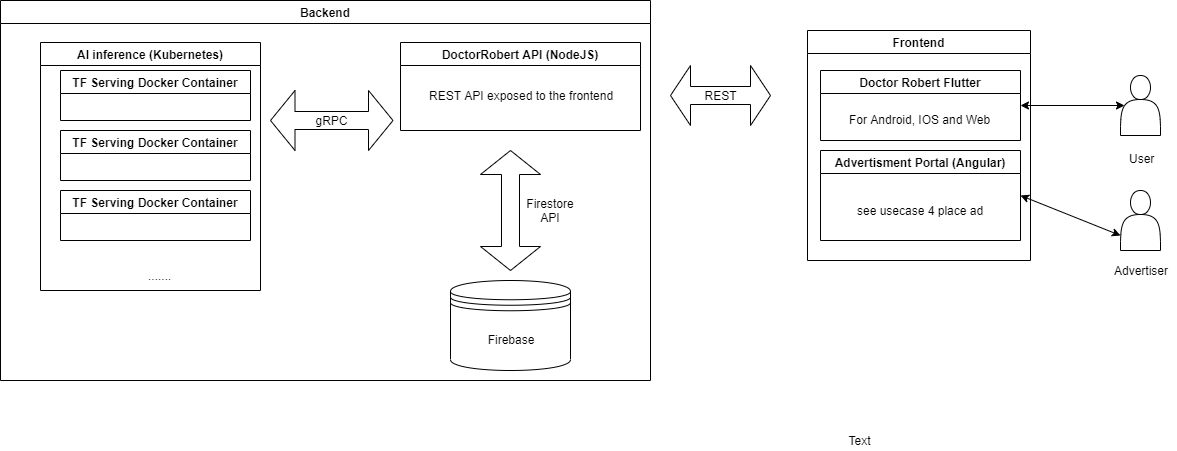
\includegraphics[scale=0.4]{SystemSpec/Usecases/Diagrams/DoctorRobertArchitecture.png}
    \caption{Illustration of the system}
    \label{fig:my_label}
\end{figure}



\subsection{Backend}

The backend consists of the following components.

\begin{itemize}
    \item AI inference/Kubernetes Cluster
    
    A Kubernetes cluster consisting of independent TensorFlow Serving Docker container will handle the computational expensive task of inferring the answer to the users query. TensorFlow Serving is a high-performance serving solution for machine learning models. Kubernetes will distribute the workload evenly between the containers and, if needed, dynamically create new ones. 
    
    \item DoctorRobert API Server/
    
    The goal of this component is to handle REST calls from the frontend. If the user requests a diagnosis for his or her symptom description, this part of the system will delegate the task via gRPC to the Kubernetes Cluster. Futhermore, the user management will be done by this server, executing the well known CRUD functionality on the Firestore database.
    
    \item Firebase's Firestore
    
    Firestore is a NoSQL database of Google's Firebase application-development suit. The communication with this cloud-service storage will be done via googles API and will only happen on the API server.
    
\end{itemize}

\subsection{Frontend}

\begin{itemize}
    \item DoctorRobert healthcare assistant
    
    The main application will be realized in flutter. This is the interface for the user.
    
    \item Advertiser Portal
    
    An Angular app for interactions with the backend regarding advertisement. This is the interface for the advertiser.
\end{itemize}

\pagebreak

\section{Acceptance Criteria}

\subsection{Acceptance Criteria 01: Get Diagnosis}
\subsubsection{Text}
\begin{tabular}{|p{.2\linewidth}|p{.65\linewidth}|}
\hline 
\cellcolor[gray]{0.5}\textcolor{white}{Steps} & \cellcolor[gray]{0.5}\textcolor{white}{Expected behaviour} \\ \hline
Use Case 1: Enter Symptoms & The user enters their symptoms and complaints, in actual spoken language. \\ \hline
Use Case 3: Get Diagnosis & Based on the user's input a certain diagnosis will be returned. If the user where to enter something nonsensical, a nonsensical answer will return.  \\ \hline
\end{tabular}

\subsubsection{Text and Picture}
\begin{tabular}{|p{.2\linewidth}|p{.65\linewidth}|}
\hline 
\cellcolor[gray]{0.5}\textcolor{white}{Steps} & \cellcolor[gray]{0.5}\textcolor{white}{Expected behaviour} \\ \hline
Use Case 1: Enter Symptoms & The user enters symptoms related to skin diseases, in actual spoken language. \\ \hline
Use Case 3: Get Diagnosis & The user gets an diagnosis and is asked to take a picture of their skin irrationality to further improve the diagnosis and make it more accurate. \\ \hline
Use Case 2: Scan Skin & The user takes a picture and submits it for further processing. \\ \hline
Use Case 3: Get Diagnosis & Now the user gets an accurate diagnosis about their skin related issue. \\ \hline
\end{tabular}

\subsubsection{Add Advertisement}
\begin{tabular}{|p{.2\linewidth}|p{.65\linewidth}|}
\hline 
\cellcolor[gray]{0.5}\textcolor{white}{Steps} & \cellcolor[gray]{0.5}\textcolor{white}{Expected behaviour} \\ \hline
Use Case 3: Get Diagnosis & An appended message will be sent along with the original one, containing credentials and further information about the advertiser, if enough keywords match.  \\ \hline
\end{tabular}

\subsection{Acceptance Criteria 02: Verify Advertiser}

\begin{tabular}{|p{.2\linewidth}|p{.65\linewidth}|}
\hline 
\cellcolor[gray]{0.5}\textcolor{white}{Steps} & \cellcolor[gray]{0.5}\textcolor{white}{Expected behaviour} \\ \hline Use Case 4: Request Verification &  Somebody who wants to have the opportunity to place ads on our app, requests a verification to be an advertiser on our website. \\ 
\hline Use Case 5: Verify Advertiser & An admin reviews the verification and either grants the requester advertiser status or rejects it. \\ 
\hline
\end{tabular}


\subsection{Acceptance Criteria 03: Place Advertisement}
\begin{tabular}{|p{.2\linewidth}|p{.65\linewidth}|}
\hline 
\cellcolor[gray]{0.5}\textcolor{white}{Steps} & \cellcolor[gray]{0.5}\textcolor{white}{Expected behaviour} \\ \hline
Use Case 6: Place Ad & An advertiser pays a certain amount in advance to promote himself, as long as the payment goes through. A small fee will be charged from his stored money every time he was advertised. \\ \hline
\end{tabular}
\end{document}